%\addcontentsline{toc}{chapter}{State transitions}\label{ch:StateTransitions}
\chapter{State transitions}
\label{ch:StateTransitions}

\begin{figure}[!htb]
\centering

\begin{tikzpicture}[->,>=stealth',shorten >=1pt,auto,node distance=8cm,semithick]
  \tikzstyle{every state}=[fill=red,draw=none,text=white]

  \node[initial,state] (A)                    {$A$};
  \node[state]         (B) [above right of=A] {$B$};
  \node[state]         (C) [below right of=B] {$C$};
  \node[state]         (D) [below right of=A] {$D$};

  \path (A) edge    [bend left]          node {$\alpha \wedge \beta$} (B)
        
        (B) edge [bend left]  node {} (A)
        
        (B) edge  [bend left] node {$\alpha \wedge \beta \wedge \gamma \wedge \delta$} (C)
        
        (B) edge [bend left] node [near end] {$\alpha \wedge \beta \wedge \gamma \wedge \delta \wedge \epsilon$} (D)
        
        (C) edge              node {} (A)
        (C) edge  [bend left] node [near start,above=10pt] {$\alpha \wedge \beta$} (B)
        
        
        (C) edge [bend left] node {$\alpha \wedge \beta \wedge \gamma \wedge \delta \wedge \epsilon$} (D)
        (D) edge [bend left]  node [near start] {$\alpha \wedge \beta$} (B)
        (D) edge [bend left] node {} (A);
        
\end{tikzpicture}
\caption{State transition diagram. The key to the symbols used for the transition conditions can be found in table \ref{tab:StateTransitionDiagramKey}.} \label{fig:StateTransitionDiagram}
\end{figure}

\ac{NAMURU} employs a number of different tracking loops which are chosen depending on the current state. A state transition diagram can be seen in figure \ref{fig:StateTransitionDiagram}. In this diagram, 4 different states are visible. This thesis focuses on the carrier tracking loops, so a simplifying assumption is made that the receiver is always perfectly tracking the code phase. 

Given the robustness of the code phase tracking loops, this is a reasonable assumption. In reality however, the receiver is initially in a acquisition state, where a delay doppler map is computed, in order to try and produce a rough estimate of the code and carrier phase.  An example of a delay doppler map can be seen in figures \ref{fig:DelayDopplerMap} and \ref{fig:DelayDopplerMapSubsection}.


\begin{table}[!htb]
\centering
\begin{tabular}{|l|l|}
\hline
\rowcolor[HTML]{C0C0C0} 
Condition & Description                                                 \\ \hline
$\alpha$    & State A for  $\geq$ 256ms                                     \\ \hline
\rowcolor[HTML]{EFEFEF} 
$\beta$     & FLL error $\leq$ 30 $\degree$                                  \\ \hline
$\gamma$    & State B for $\geq$ 256ms                                      \\ \hline
\rowcolor[HTML]{EFEFEF} 
$\delta$    & 20/32 of last measurements have phase error $\leq$ 30 $\degree$ \\ \hline
$\epsilon$  & State B for $\geq$ 256ms                                      \\ \hline
\end{tabular}
\caption{State transition diagram key.}
\label{tab:StateTransitionDiagramKey}
\end{table}

\section{State A}
After acquisition, the receiver will achieve code lock almost immediately, at which point the receiver is in state A. Once the receiver is in state A, a FLL is initiated. The FLL is very simple in structure, consisting of a single proportional arm, with a gain of 0.125. As the receiver has not undergone bit alignment, the loop filter needs to be relatively insensitive to bit transitions. As alluded to before, a FLL with a finite gain is unable to completely remove the frequency error, however the goal of the pure FLL state is to get the receiver closer in frequency.

As alluded to before, the lock range of the receiver is given by:

\begin{equation}
\frac{-1}{2T} < f < \frac{1}{2T}
\end{equation}

When $T = 0.004$, the FLL has a locking range of $\pm 125Hz$. At the L1 frequency, 125Hz corresponds to $23.8ms^{-1}$. Accelerating at 15g ($147ms^{-2}$), the receiver needs to start locking within $\approx 160ms$, otherwise the doppler frequency will be outside the locking range.

\section{State B}
Once the receiver has been in the A state for at least 256ms, and once a filtered version of the frequency error is less then $30 \degree$, then the receiver transitions into state B. State B uses a second order PLL with a first order FLL. State B is also known as "Frequency lock".


\section{State C}
Once the receiver has been in state B for at least 256ms, and if at least 20 of the past 32 measurements have a phase error of less than 30 degrees, then the receiver transitions to state C. State C has exactly the same loop structure as state B, however the receiver is now considered to be in "phase lock", and data extraction can begin.

\section{State D}
Once the receiver has been in state C for at least 1280ms, the receiver transitions to state D. State D has a 3rd order PLL and a 2nd order FLL, and forms the focus of this thesis. While any of the PLLs can be used to decode the incoming data, only the 3rd order PLL is insensitive to acceleration.  

\begin{figure}[!htb] 
    \centering
    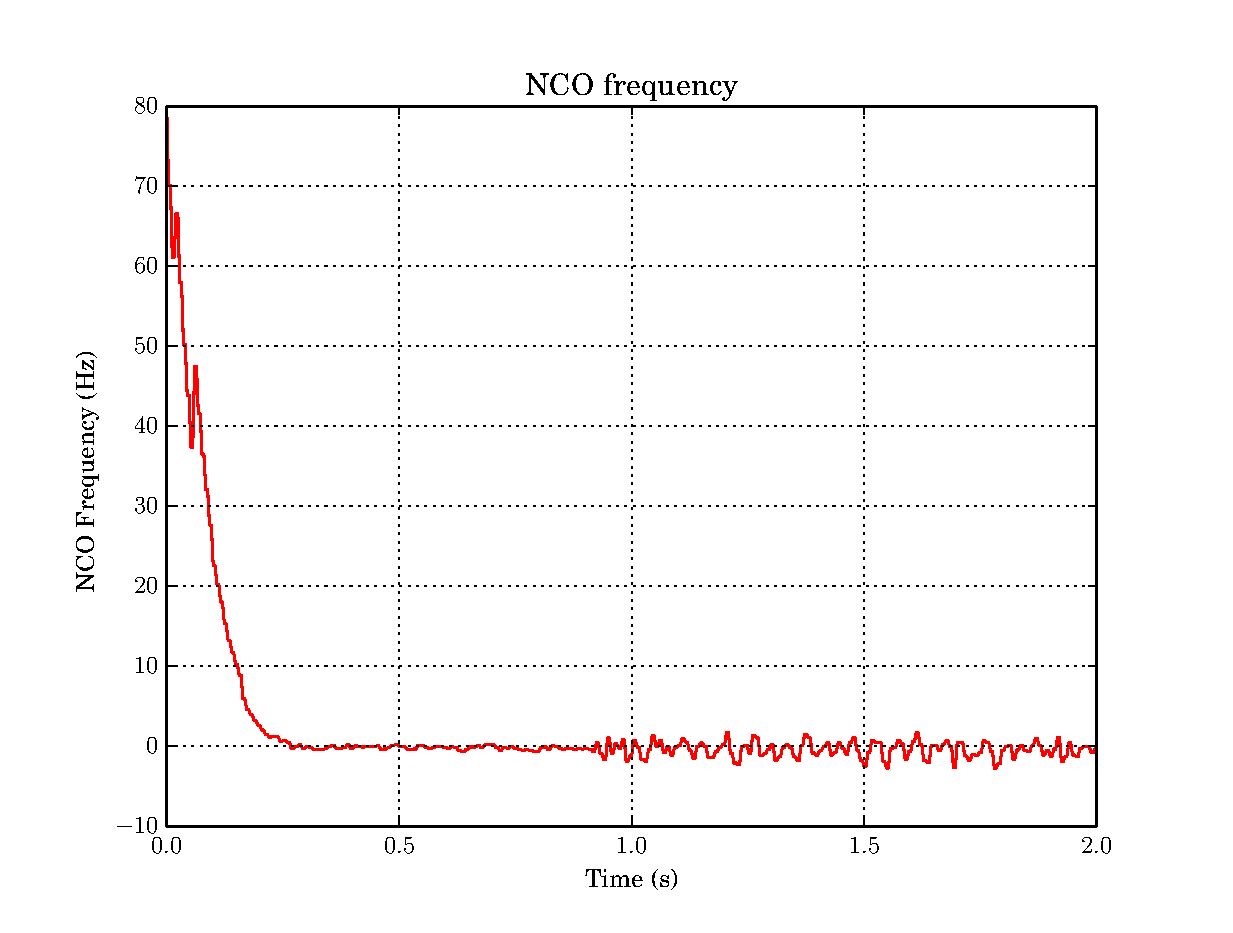
\includegraphics[width=1\textwidth]{LoopStates.eps} 
    \caption{This figure visualises the process of achieving phase lock. Initially, there is a 80Hz frequency difference between the local oscillator and the carrier frequency. At approximately 900ms, the transition to a larger bandwith tracking loop can be observed. }
    \label{fig:LoopStatesGraph}
\end{figure}


\section{Analysis}
Careful analysis of the state transitions reveals some salient insights. In particular, it is possible to transition directly from state B to state D, if the receiver has previously been in state C. This transition is intriguing, given that the GPS should ideally be agnostic to it's state history. After a careful discussion with Dr Glennon, it became apparent that this quirk was an unintended bug in the firmware.

Further analysis identifies the potential to radically simplify the state transitions, in conjunction with modifying the structures and loop bandwidths employed in the different states. From an intuitive perspective, the goal of the firmware should be to attempt to move the receiver into a state which produces more accurate measurements. This philosophy is illustrated in the movement from simple FLL which eliminates gross errors to a combination  PLL/FLL. However, the final step to a 3rd order PLL / 2nd order FLL is perplexing. 

In particular, the noise bandwidth $B_n$ of state D (32,10) is larger than that of state B\&C (18,1). Hence, in the case that the PLL/FLL in state D fails, the receiver will drop down to state B, which will immediately fail due to it's higher sensitivity to dynamics. At this point, the receiver will drop into state A. Conversely, this suggests that it should be possible to transition  directly from state A to state D, without the requirements for states B \& C. 

This leads to the conclusion that states B \& C are potentially vestigial, and should be removed. An alternative point of view is that the PLL \& FLL $B_n$ of state B \& C should be significantly increased, and state D should be converted from a PLL \& FLL to a pure PLL, provided that state C is capable of sufficiently reducing the frequency error so that it is within the locking range of state D's PLL.

